% slide 8
\begin{frame}
    \frametitle{Programación Reactiva}
    \begin{itemize}
        \item<1-> \textbf{Reactividad}: cuando los \textit{outputs} reaccionan a los cambios de los \textit{inputs}.
        \item<2-> Cuando una variable \codigo{x} cambia su valor, todo lo relativo a \codigo{x} también cambia su valor. 
        \item<3->  R usa programación reactiva a través de Shiny
        \item<4->[]
        \begin{figure}[h!]
            \centering
                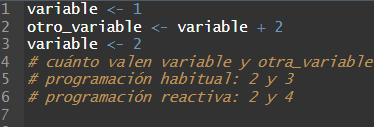
\includegraphics[scale=0.6]{Imagenes/03_Reactividad.png}
            \label{fig:fig3}
            \end{figure} 
  \end{itemize}
\end{frame}